Comecei por treinar uma árvore de decisão simples, carregando outro \textit{dataset} para servir de conjunto de dados de teste.

\begin{figure}[H]
    \centering
    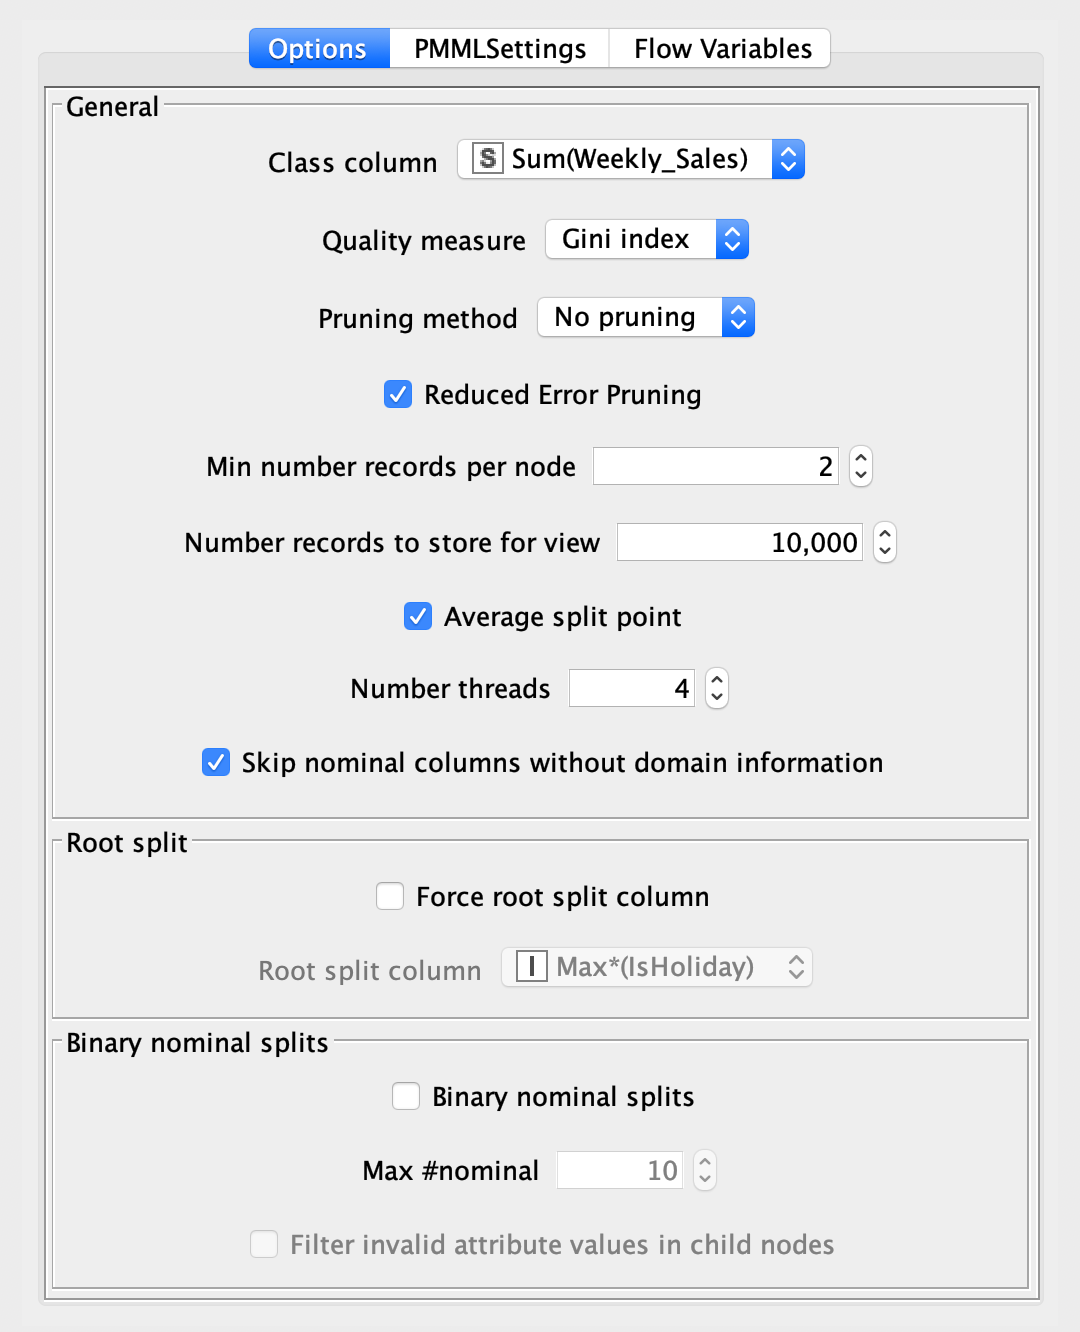
\includegraphics[scale=0.4]{Images/T3_a.png}
    \caption{Nodo Decision Tree Learner}
\end{figure}

\begin{figure}[H]
    \centering
    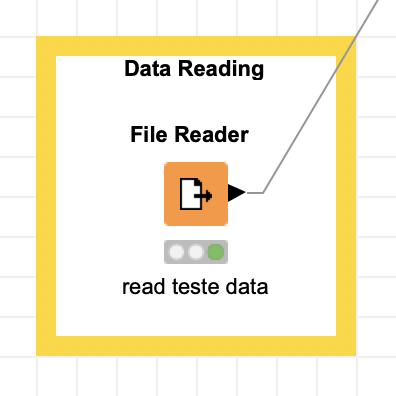
\includegraphics[scale=0.5]{Images/T3_b1.png}
    \caption{Leitura do dataset de teste}
\end{figure}

\begin{figure}[H]
    \centering
    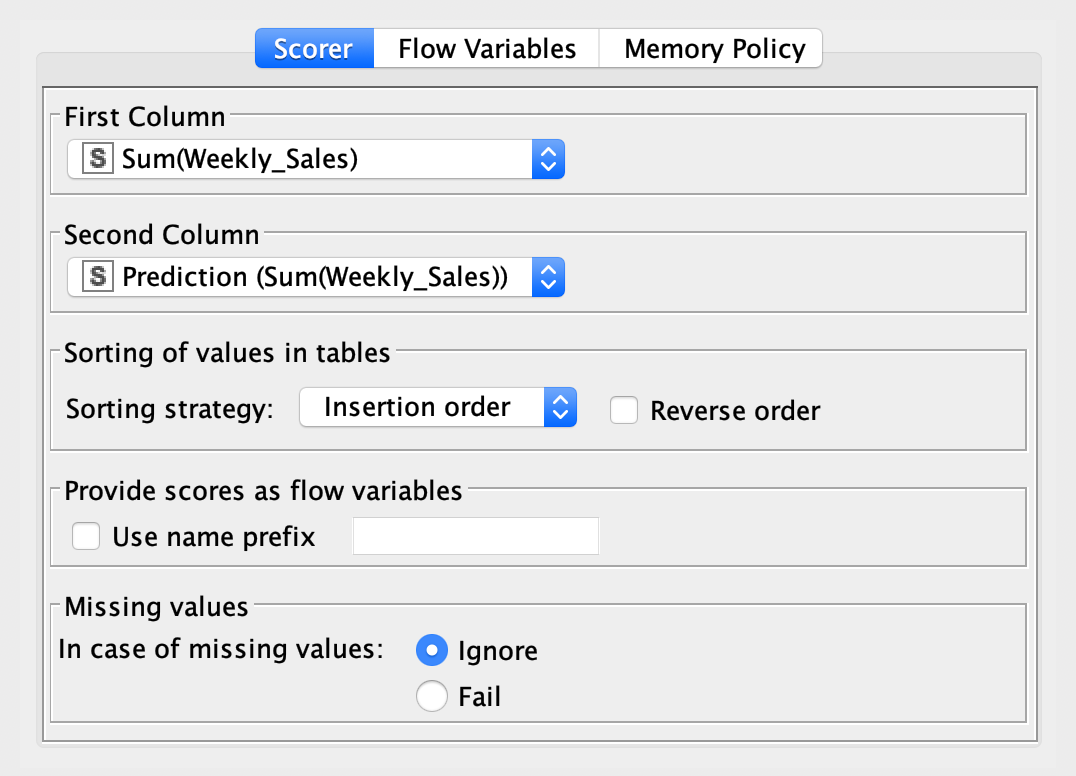
\includegraphics[scale=0.4]{Images/T3_c1.png}
    \caption{Nodo Scorer}
\end{figure}

Obtive a seguinte matriz de confusão resultante do nodo \textit{Scorer}.

\begin{figure}[H]
    \centering
    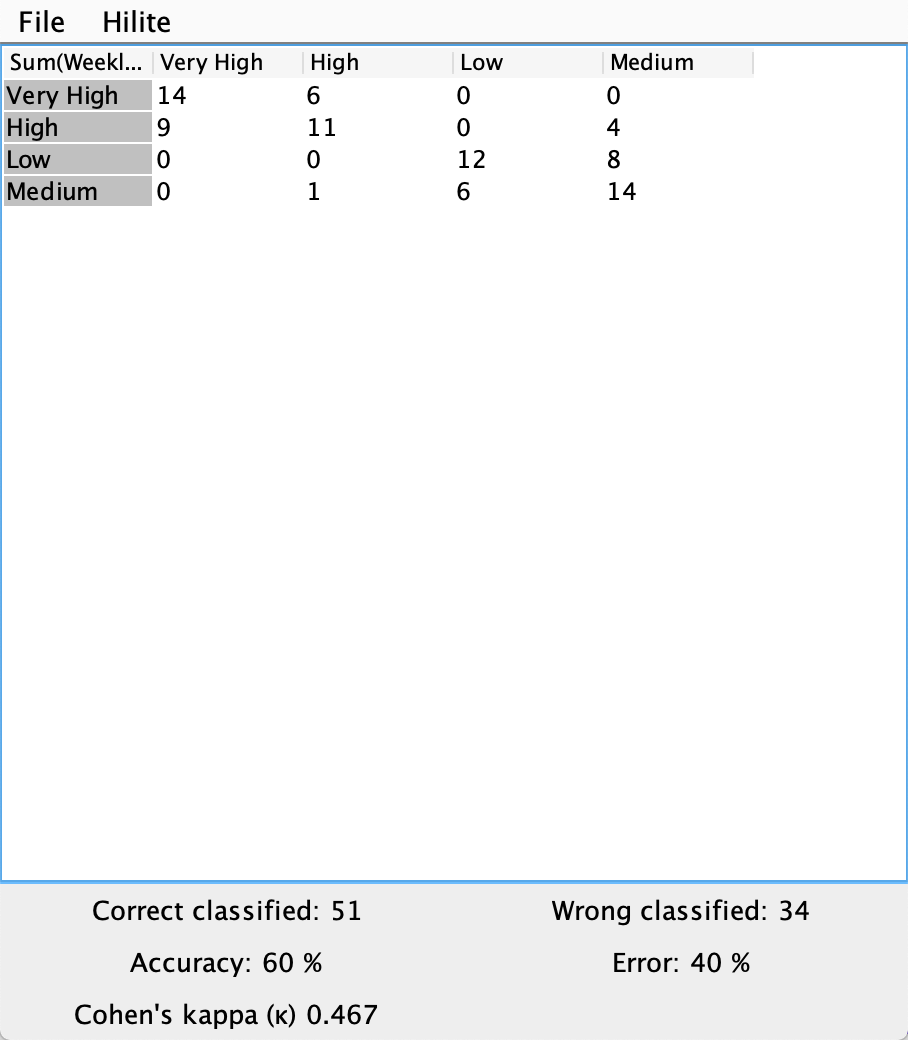
\includegraphics[scale=0.4]{Images/T3_c2.png}
    \caption{Matriz de confusão}
\end{figure}

\clearpage

O seguinte \textit{workflow} representa todos os passos realizados para esta tarefa.

\begin{figure}[H]
    \centering
    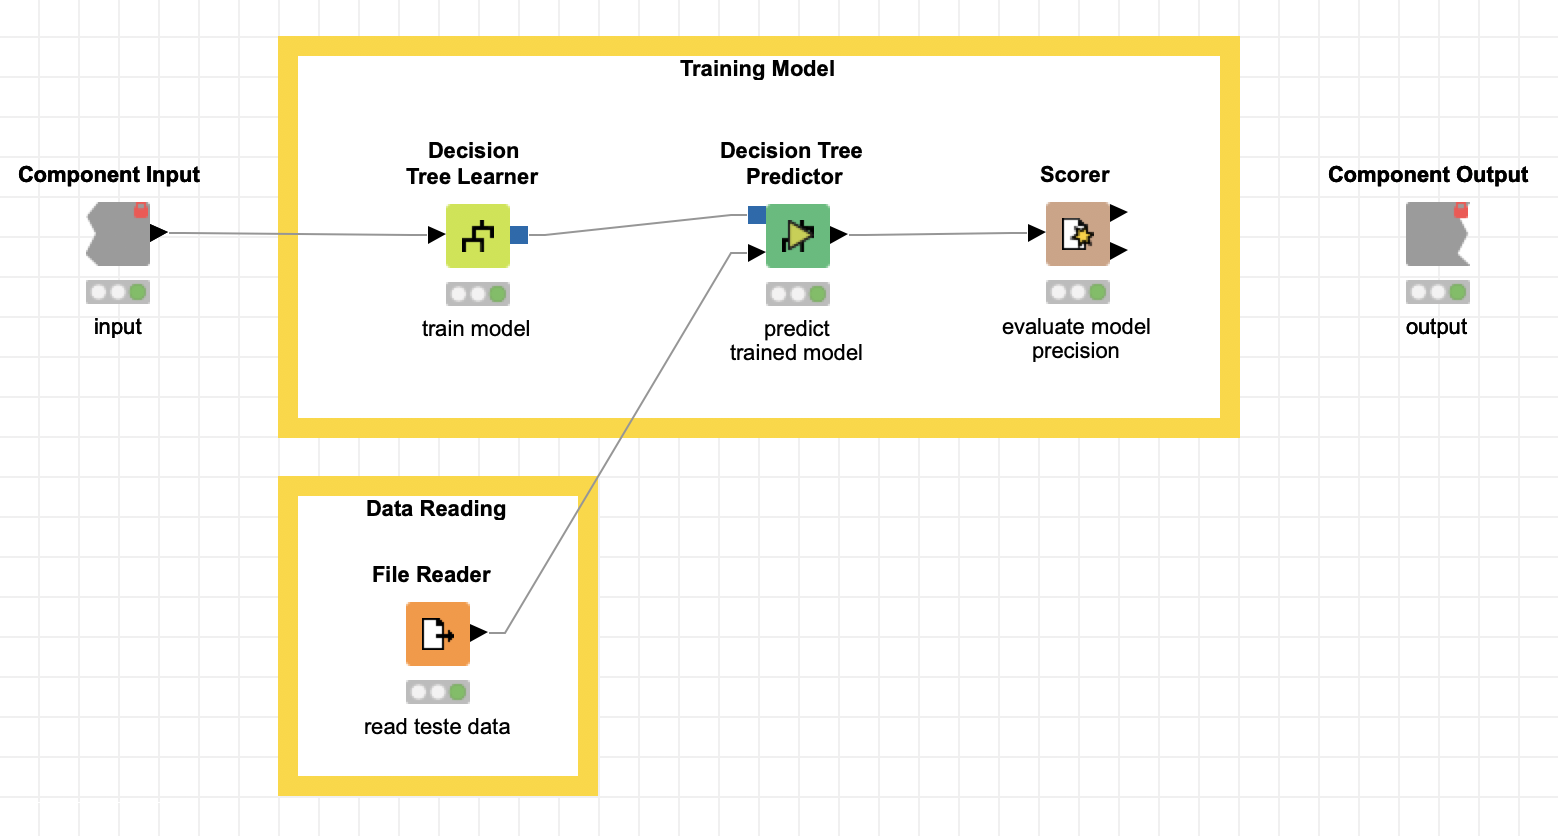
\includegraphics[scale=0.4]{Images/T3.png}
    \caption{Workflow}
\end{figure}